\scanpage{12}
a) Les catégories de structures a) b) introduites précédemment définissent-elles des \uline{champs} sur $S_{\mathrm{zar}}$ ?
\margin{oui si on suppose que les \deleted{\unsure{hom}}
\deleted{$\unsure{H_0(\ell),H_0(\check\ell'[1])\simeq0}$}
\inserted{$\unsure{H_1(\ell_{\bullet})\mathbin{-}H_1(\ell'_{\bullet})}$}
\deleted{\unsure{et soient localement}}
\diagram{\begin{tikzcd}0\arrow[r]&\unsure{t^*}\arrow[r,dash]&\omega\end{tikzcd}}
avec $\unsure{\omega}\text{ et }\omega^*\ t\ t^*$ loc. libres}
\figure{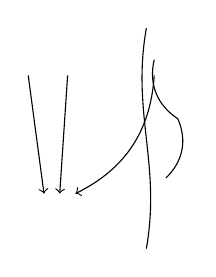
\begin{tikzpicture}\draw(0,0) to[out=80,in=260] (0,2.8);\draw[->](-1.5,2.2)--(-1.3,.7);\draw[->](-1,2.2)--(-1.1,.7);\draw[->](.1,2.2) to[bend left=30](-.9,.7);\draw(.1,2.4) to[bend right=35](.4,1.65) to[bend left=35](.25,.9);\end{tikzpicture}}

b) le foncteur ``oubli partiel'' \inserted{(de $\mathcal C$ de b))} allant vers les cristaux $\mathcal M$ sur $S_{\mathrm{cris}}/\mathbb F_p$ est-il \uline{fidèle} ?

c) Le foncteur naturel $\unsure{\mathcal M_\omega|\mathcal M\to}$ des modules loc. libres $\omega$ sur $S_{\mathrm{zar}}$, avec $F_\omega,V_\omega$, vers les structures a), b), est-il pleinement fidèle (NB il est fidèle); l'est-il du moins \deleted{\unsure{pour de}} \deleted{si $F_\omega=0$} sur la sous-catégorie définie par $F_\omega=0$; l'est il \inserted{$\operatorname{Ker}F=\operatorname{Im}V$} ?

d) Peut-on à $(\omega,F_\omega,V_\omega)$ associer un schéma en groupes fini loc libre sur $S$ ?
\mspage{11}
